\documentclass[a4paper,twoside]{article}
\usepackage[T1]{fontenc}
\usepackage[bahasa]{babel}
\usepackage{graphicx}
\usepackage{graphics}
\usepackage{float}
\usepackage[cm]{fullpage}
\pagestyle{myheadings}
\usepackage{etoolbox}
\usepackage{setspace} 
\usepackage{lipsum} 
\usepackage{listings}
\setlength{\headsep}{30pt}
\usepackage[inner=2cm,outer=2.5cm,top=2.5cm,bottom=2cm]{geometry} %margin
% \pagestyle{empty}

\makeatletter
\renewcommand{\@maketitle} {\begin{center} {\LARGE \textbf{ \textsc{\@title}} \par} \bigskip {\large \textbf{\textsc{\@author}} }\end{center} }
\renewcommand{\thispagestyle}[1]{}
\markright{\textbf{\textsc{Laporan Perkembangan Pengerjaan Skripsi\textemdash Sem. Ganjil 2018/2019}}}

\onehalfspacing
 
\begin{document}

\title{\@judultopik}
\author{\nama \textendash \@npm} 

%ISILAH DATA BERIKUT INI:
\newcommand{\nama}{Matthew Ariel Wangsit}
\newcommand{\@npm}{2015730010}
\newcommand{\tanggal}{20/11/2018} %Tanggal pembuatan dokumen
\newcommand{\@judultopik}{Reduksi Big Data dengan Algoritma Clustering untuk Spark} % Judul/topik anda
\newcommand{\kodetopik}{VSM4502}
\newcommand{\jumpemb}{1} % Jumlah pembimbing, 1 atau 2
\newcommand{\pembA}{Veronica Sri Moertini}
\newcommand{\pembB}{-}
\newcommand{\semesterPertama}{45 - Ganjil 18/19} % semester pertama kali topik diambil, angka 1 dimulai dari sem Ganjil 96/97
\newcommand{\lamaSkripsi}{1} % Jumlah semester untuk mengerjakan skripsi s.d. dokumen ini dibuat
\newcommand{\kulPertama}{Skripsi 1} % Kuliah dimana topik ini diambil pertama kali
\newcommand{\tipePR}{B} % tipe progress report :
% A : dokumen pendukung untuk pengambilan ke-2 di Skripsi 1
% B : dokumen untuk reviewer pada presentasi dan review Skripsi 1
% C : dokumen pendukung untuk pengambilan ke-2 di Skripsi 2

% Dokumen hasil template ini harus dicetak bolak-balik !!!!

\maketitle

\pagenumbering{arabic}

\section{Data Skripsi} %TIDAK PERLU MENGUBAH BAGIAN INI !!!
Pembimbing utama/tunggal: {\bf \pembA}\\
Pembimbing pendamping: {\bf \pembB}\\
Kode Topik : {\bf \kodetopik}\\
Topik ini sudah dikerjakan selama : {\bf \lamaSkripsi} semester\\
Pengambilan pertama kali topik ini pada : Semester {\bf \semesterPertama} \\
Pengambilan pertama kali topik ini di kuliah : {\bf \kulPertama} \\
Tipe Laporan : {\bf \tipePR} -
\ifdefstring{\tipePR}{A}{
			Dokumen pendukung untuk {\BF pengambilan ke-2 di Skripsi 1} }
		{
		\ifdefstring{\tipePR}{B} {
				Dokumen untuk reviewer pada presentasi dan {\bf review Skripsi 1}}
			{	Dokumen pendukung untuk {\bf pengambilan ke-2 di Skripsi 2}}
		}
		
\section{Latar Belakang}

{\it Big data} adalah sebuah istilah yang menggabarkan volume data yang besar, baik data yang terstruktur maupun data yang tidak terstruktur. Data-data tersebut memiliki potensi untuk digalih menjadi informasi yang penting. Dalam bidang {\it big data} ada  berapa tantangan seperti volume data yang besar, kecepatan aliran data masuk yang harus ditangani, dan variasi data dengan format yang berbeda. Tantangan tersebut membuat {\it traditional data-processing application software} tidak bisa memproses dan menganalisis {\it big data}. Munculah teknologi-teknologi seperti Hadoop dan Spark yang khusus untuk menangani {\it big data}. 

{\it Big data} akan lebih mudah dianalisis dan diterapkan teknik-teknik {\it data-mining} ketika volume {\it big data} tersebut telah direduksi. Dengan mereduksi data, kita bisa menghemat biaya transfer data, {\it disk space}, dan jumlah data yang diproses. Hasil dari reduksi {\it big data} harus bisa mewakili {\it the original big data} secara akurat. 

Salah satu cara mereduksi data adalah dengan menggunakan algoritma {\it Clustering Agglomerative}. Algoritma tersebut cocok untuk data yang tidak memiliki atribut yang terlalu banyak. {\it Science journal} berjudul {\it Big Data Reduction Technique using Parallel Hierarchical Agglomerative Clustering} sudah meneliti algorima {\it Clustering Agglomerative} berbasis MapReduce pada Hadoop. Sudah terbukti bahwa data yang direduksi dengan algoritma tersebut bisa mewakili data secara keseluruhan. Algoritma {\it Clustering Agglomerative} bekerja dengan membiarkan setiap objek membentuk {\it sub-cluster}. Kemudian, {\it sub-cluster} akan di gabung dengan {\it sub-cluster} lainya secara iterasi sampai terbentuknya {\it single cluster}. {\it single cluster} akan menjadi akar dari {\it hierarchy}, {\it cluster} tersebut digabung dengan {\it cluster} terdekat bedasarkan jarak minimum atau kesamaan.

Walau reduksi data dengan algoritma {\it Agglomerative} berbasis MapReduce pada Hadoop bisa mewakili {\it the original big data} secara akurat, MapReduce pada Hadoop memiliki kekurangan. Kekurangan MapReduce adalah dalam melakukan {\it itterative processing}, MapReduce akan menuliskan hasil sementara iterasi kepada disk. Hal ini membuat MapReduce lama dalam mengerjakan proses iterasi. Algoritma {\it Agglomerative} yang mengandung banyak iterasi kurang baik ketika diimplementasikan pada Hadoop MapReduce, hasil sementara akan dituliskan kepada disk berulang kali.

Spark adalah {\it distributed cluster-computing framework} yang bisa menggantikan MapReduce beserta kekurangannya. {\it In-memory processing} Spark mengalahkan kecepatan pemrosesan pada Hadoop MapReduce. Karena proses dilakukan pada RAM, kecepatan pemrosesan akan jauh lebih cepat. Tidak hanya itu, kecepatan proses iterasi meningkat karena  hasil sementara tidak harus ditulis kepada disk. Spark {\it Resilient Distributed Datasets} (RDDs) memungkinkan {\it multi map operation} pada memori.

Pada skripsi ini, akan dibangun sebuah perangkat lunak yang dapat mereduksi {\it big data}. Perangkat lunak tersebut akan dibangun menggunakan framework terdistribusi Spark dan mengimplementasikan algoritma {\it Agglomerative} yang khusus dikustomisasi untuk lingkungan Spark. Perangkat lunak akan menampilkan hasil reduksi dalam format visual dan tabel. Dengan menggunakan Spark, waktu proses reduksi data akan lebih cepat dibanding MapReduce.


\section{Rumusan Masalah}

Dari latar belakang di atas maka dapat dibentuk rumusan masalah adalah sebagai berikut:
\begin{enumerate}

\item Bagaimana cara kerja algoritma {\it Agglomerative Clustering} berbasis MapReduce untuk mereduksi {\it big data}?

\item Bagaimana cara mengkustomisasi dan mengimplementasikan aggloritma {\it Agglomerative Clustering} pada sistem tersebar Spark?

\item Bagaimana mengukur kinerja hasil dari implementasi dari algoritma {\it Agglomerative Clustering} pada sistem tersebar Spark?

\item Bagaimana cara mempresentasikan data yang telah direduksi agar dapat diinterpretasikan pengguna dengan mudah?

\end{enumerate}



\section{Tujuan}

Dari rumusan masalah di atas maka tujuan dari penelitian adalah sebagai berikut:
\begin{enumerate}

\item Mempelajari cara kerja algoritma  {\it Agglomerative Clustering} berbasis MapReduce untuk mereduksi {\it big data}.

\item Mengkustomisasi dan mengimplementasikan algoritma {\it Agglomerative Clustering} pada lingkungan Spark.

\item Melakukan eksperimen pada lingkungan sistem tersebar Spark untuk mengukur kinerja algoritma lingkungan Spark.

\item Membuat modul program yang dapat memudahkan pengguna menginterpretasikan data yang telah direduksi.

\end{enumerate}




\section{Detail Perkembangan Pengerjaan Skripsi}

Detail bagian pekerjaan skripsi sesuai dengan rencan kerja/laporan perkembangan terkahir :

	\begin{enumerate}
	
		\item \textbf{Melakukan studi literature mengenai \textit{big data}}\\
		{\bf Status :} baru ditambahkan pada semester ini\\
		{\bf Hasil :} {\it Big data} adalah istilah yang menggambarkan kumpulan data dalam jumlah yang sangat besar, baik data yang terstruktur maupun data yang tidak terstruktur. Data-data tersebut menyimpan informasi yang bisa dianalisis dan diproses untuk memberikan wawasan kepada organisasi atau perusahaan. Data-data tersebut dihasilkan dari satu atau lebih sumber  dengan kecepatan yang tinggi dan format yang berbeda-beda. Karena ukuran dan keberagaman data, {\it big data} menjadi sulit untuk ditangani atau diproses jika hanya menggunakan manajemen basis data atau aplikasi pemrosesan data traditional.\\


\begin{figure}[H]
    \centering  
    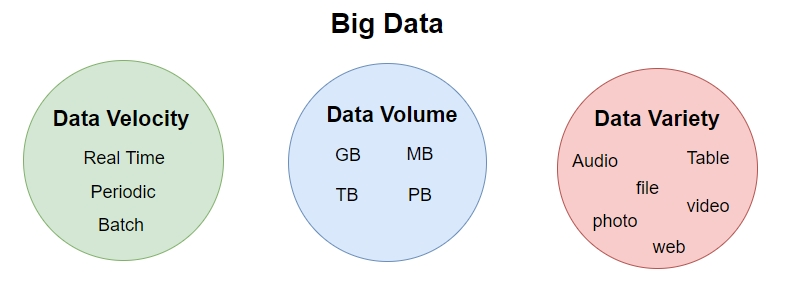
\includegraphics[scale=0.7]{bigdata}  
    \caption[Gambar {\it big data volume, velocity, variety} ]{Gambar {\it big data volume, velocity, variety}} 
    \label{fig:bigdata} 
\end{figure}

Berdasakan gambar diatas (Gambar ~\ref{fig:bigdata}), \textit{big data} memiliki tiga karakteristik diantaranya:

\begin{enumerate}

\item {\it Volume}: {\it big data} memiliki jumlah data yang sangat besar sehingga dalam proses pengolahan data dibutuhkan suatu penyimpanan yang besar dan dibutuhkan analisis yang lebih spesifik.

\item {\it Velocity}: {\it big data} memiliki aliran data yang sangat cepat.

\item {\it Variety}: {\it big data} memiliki bentuk format data yang beragam baik terstruktur ataupun tidak terstruktur dan bergantung pada banyaknya sumber data.

\end{enumerate}

{\it Big data} sangat bermanfaat ketika diterapkan di berbagai macam bidang seperti bisnis, kesehatan, pemerintahan, pertanian dan lainya. Ketika organisasi mampu menggabungkan jumlah data besar yang dimilikinya dengan analisis bertenaga tinggi, organisasi dapat menyelesaikan tantangan dan masalah yang berhubungan dengan bisnis seperti:

\begin{enumerate}

\item Menentukan akar penyebab kegagalan untuk setiap masalah bisnis.

\item Menghasilkan informasi mengenai titik penting penjualan berdasarkan kebiasaan pelanggan dalam membeli.

\item Menghitung kembali seluruh risiko yang ada dalam waktu yang singkat.

\item Mendeteksi perilaku penipuan yang dapat mempengaruhi organisasi.

\end{enumerate}
		


		\item \textbf{Melakukan studi literatur mengenai Hadoop}\\
		{\bf Status :} Ada sejak rencana kerja skripsi \\
		{\bf Hasil :} Hadoop dikembangkan oleh Doug Cutting dan Mike Cafarella pada tahun 2005 yang saat itu bekerja di Yahoo. Nama Hadoop berdasarkan mainan 'Gajah' anak dari Doug Cutting. Hadoop adalah sebuah framework atau platform open source berbasis Java. Hadoop memiliki kemampuan untuk penyimpanan dan memproses data dengan skala yang besar secara terdistribusi pada {\it cluster} yang terdiri dari perangkat keras komoditas. Hadoop menggunakan teknologi Google MapReduce dan Google File System (GFS) sebagai fondasinya ~\cite{tomwhite:01:htdg}. Beberapa karakteristik yang dimilki Hadoop adalah sebagai berikut:


\begin{enumerate}

\item {\it Open Source}: Hadoop merupakan proyek {\it open source} dan kodenya bisa dimodifikasi sesuai kebutuhan. 

\item {\it Distributed computing}: Data disimpan secara terdistribusi pada HDFS di berbagai {\it cluster} dan data diproses secara parallel pada node-node di {\it cluster}.

\item {\it Fast}: Hadoop sangat baik untuk melakukan {\it high-volume batch processing} karena kemampuannya melakukannya secara parallel.

\item {\it Fault Tolerance}: Hadoop melakukan duplikasi data di beberapa node yang berbeda. Ketika sebuah node gagal memproses data, node yang memiliki duplikat data bisa mengantikanya untuk memproses data tersebut.

\item {\it Reliability}: Kegagalan mesin bukan masalah bagi Hadoop karena adanya duplikasi data.


\item {\it High availability}: Data dapat diambil dari sumber yang lain meskipun kegagaln mesin karena adanya duplikasi data.

\item {\it Scalability}: Hadoop dengan sangat mudah dapat menambahkan node yang lebih banyak kedalam {\it cluster}.

\item {\it Flexibility}: Hadoop dapat menangani data terstruktur maupun data tidak terstruktur. 

\item {\it Economic and cost effective}: Hadoop tidak terlalu mahal karena berjalan pada {\it cluster} terdiri dari perangkat keras komoditas.

\item {\it Easy to use}: Hadoop mempermudah pengguna dalam merancang program parallel. Hadoop sudah menangani hal-hal terakit {\it distributed computing}.

\item {\it Data locality}: Algoritma MapReduce akan didekatkan kepada {\it cluter} dan tidak sebaliknya. Ukuran data yang besar lebih sulit untuk dipindahkan dibanding ukuran algoritma yang kecil.


\end{enumerate}

\begin{figure}[H]
    \centering  
    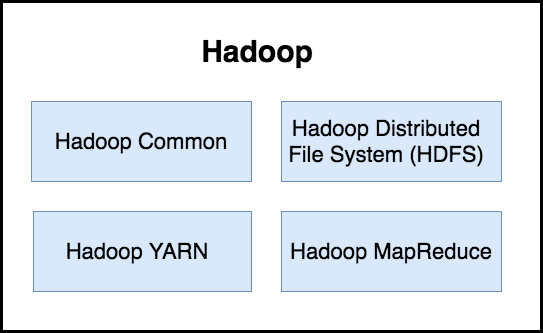
\includegraphics[scale=0.5]{hmodule}  
    \caption[Gambar modul-modul Hadoop ]{Gambar modul-modul Hadoop} 
    \label{fig:hmodule} 
\end{figure}

Bedasarkan gambar diatas (Gambar ~\ref{fig:hmodule}), {\it framework} Apache Hadoop terdiri dari beberapa modul. Module-module tersebut membentuk dan membantu untuk memproses data yang bersakala besar. Modul-modul itu diantaranya adalah:

\begin{enumerate}
\item Hadoop Common, module ini mengandung {\it library} dan {\it tools} yang dibutuhkan module Hadoop lainnya.

\item Hadoop Distributed File System (HDFS), sebuah \textit{file-system} terdistribusi milik Hadoop untuk penyimpanan data.

\item Hadoop YARN, {\it resource-management platform} yang bertanggung jawab untuk mengatur sumber daya pada {\it cluster}.

\item MapReduce, sebuah programming model untuk pemrosesan skala besar.

\end{enumerate}

\textbf{Master Slave Architecture Pada Hadoop}

\begin{figure}[H]
    \centering  
    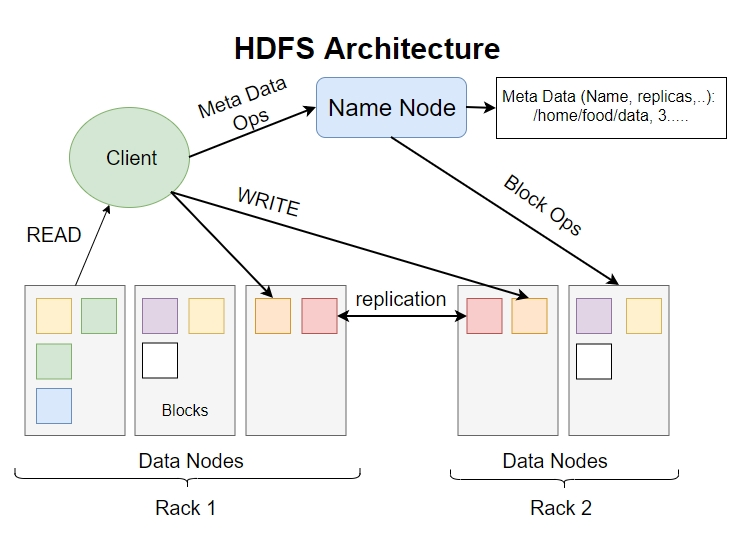
\includegraphics[scale=0.6]{hdfshadoop}  
    \caption[Gambar arsitektur HDFS]{Gambar arsitektur HDFS} 
    \label{fig:hdfshadoop} 
\end{figure}

Hadoop meimplementasikan {\it Master Slave Architecture} pada komponen primernya yaitu HDFS dan MapReduce. Bedasarkan  (Gambar ~\ref{fig:hdfshadoop}), NameNode atau disebut master node bertugas mengatur {\it file system namepsace} seperti {\it open, close, rename} file dan direktori. Selain itu, NameNode meregulasi akses user terhadap file dan mengatur block mana yang akan diolah oleh DataNode. DataNode atau bisa disebut {\it slave node} merupakan pekerja dari HDFS. DataNode bertangungjawab untuk membaca dan menulis request dari {\it file system} Hadoop. NameNode bisa melakukan block {\it create, delete,} dan {\it replicate} ketika diberi instruksi dari {\it master node}. 

\begin{figure}[H]
    \centering  
    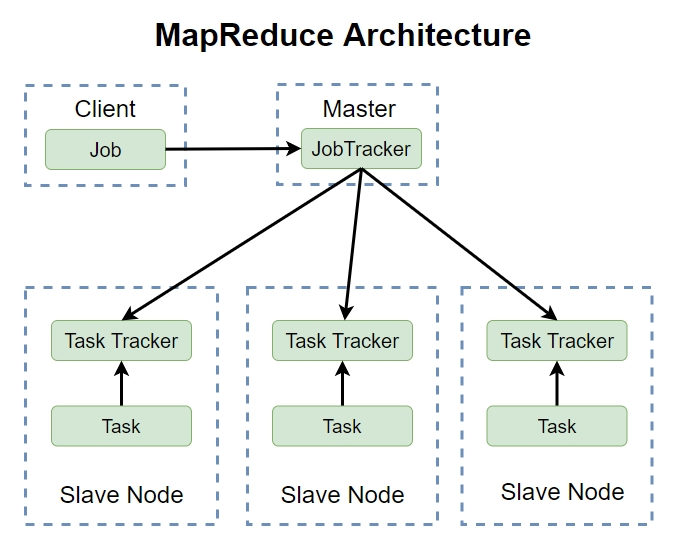
\includegraphics[scale=0.5]{mapreducehadoop}  
    \caption[Gambar arsitektur MapReduce]{Gambar arsitektur MapReduce} 
    \label{fig:mapreducehadoop} 
\end{figure}

Bisa dilihat pada (Gambar ~\ref{fig:mapreducehadoop}) yaitu arsitektur MapReduce, {\it master node} disebut JobTracker dan {\it slave node} disebut TaskTracker. JobTracker adalah jembatan antara user dan fungsi map maupun reduce. Ketika Map atau Reduce job diterima oleh JobTracker, job tersebut akan dimasukan kedalam queue dan menjalankan job sesuai urutan {it first-come/first-served}. Job yang dieksekusi akan ditugaskan kepada TaskTracker oleh JobTracker. TaskTracker atau {\it slave} menproses {\it task} yang diberikan oleh JobTracker. Pergerakan data dari fase Map ke fase Reducer ditangani oleh TaskTracker.  

\textbf{MapReduce}\\

MapReduce adalah model pemrograman untuk memproses data berukuran raksasa secara terdistribusi dan paralel dalam cluster yang terdiri atas ribuan komputer. Dalam memproses data, secara garis besar MapReduce dapat dibagi dalam dua proses yaitu proses Map dan proses Reduce. Setiap fase memiliki \textit{key-value pairs} sebagai input dan output ~\cite{tomwhite:02:htdg}. Kedua jenis proses ini didistribusikan atau dibagi-bagikan ke setiap komputer dalam suatu cluster dan berjalan secara paralel tanpa saling bergantung satu dengan yang lainnya. Proses Map bertugas untuk mengumpulkan informasi dari potongan-potongan data yang terdistribusi dalam tiap komputer dalam cluster. Hasilnya diserahkan kepada proses Reduce untuk diproses lebih lanjut. Hasil proses Reduce merupakan hasil akhir.\\

\begin{figure}[H]
    \centering  
    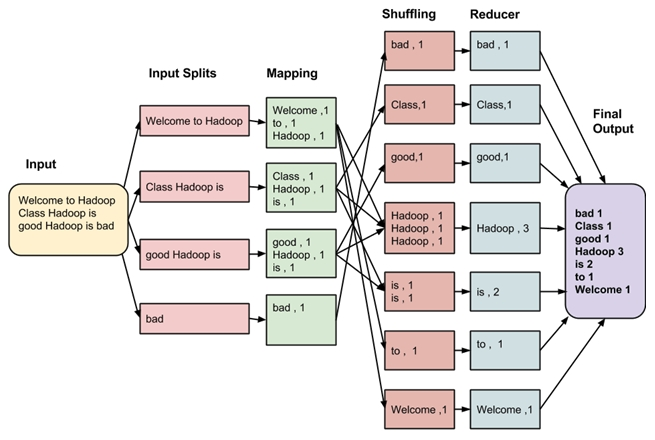
\includegraphics[scale=1]{mpstep}  
    \caption[Gambar proses MapReduce]{Gambar proses MapReduce} 
    \label{fig:mpstep} 
\end{figure}

Bedasarkan (Gambar ~\ref{fig:mpstep}) , berikut adalah langkah-langkah proses awal \textit{input} sampai akhir dari MapReduce:

\begin{enumerate}
\item \textit{Input} dibagi menjadi {\it input split} yang berukuran sama, untuk setiap input splits dibuatlah Map {\it task}.

\item Pada fase Map, data pada setiap \textit{split} akan dihitung berapa banyak kemunculan kata tersebut dan dijadikan pair <word, frequency> sebagai \textit{ouput}.

\item Setelah phase Mapping, output dari fase ini memasuki tahap Shuffling dimana tugasnya adalah untuk mengkonsolidasikan {\it records} yang relevant dari \textit{output} fase Map. Dalam contoh ini, kata-kata yang sama disatukan bersama dengan frekuensi masing-masing.

\item Terakhir adalah fase Reduce dimana \textit{ouput} dari \textit{shuffling} akan dikumpulkan. Nilai-nilai dari fase \textit{shuffling} akan digabungkan menjadi sebuah \textit{output}. \textit{Output} akan disimpan pada HDFS.

\end{enumerate}


\textbf{Hadoop Distributed File System}\\

Hadoop Distributed File System (HDFS) adalah sistem file terdistribusi yang dirancang untuk berjalan pada perangkat keras komoditas. HDFS berbeda dari sistem file terdistribusi lainnya adalah  karena sifat {\it fault tolerant} yang tinggi dan dirancang untuk digunakan pada perangkat keras biasa. HDFS menyediakan akses throughput yang tinggi ke data aplikasi dan cocok untuk aplikasi yang memiliki set data yang besar. HDFS awalnya dibangun sebagai infrastruktur untuk proyek mesin pencari web Apache Nutch.\\


Kegagalan perangkat keras sudah biasa terjadi. HDFS mungkin terdiri dari ratusan atau ribuan mesin server, masing-masing menyimpan bagian dari data {\it file sustem}. Faktanya, ada sejumlah besar komponen dan setiap komponen memiliki probabilitas kegagalan. Hal ini  menandakan bahwa beberapa komponen HDFS selalu tidak berfungsi. Oleh karena itu, deteksi kesalahan dan pemulihan otomatis yang cepat dari sistem adalah tujuan arsitektur inti dari HDFS.\\

\begin{figure}[H]
    \centering  
    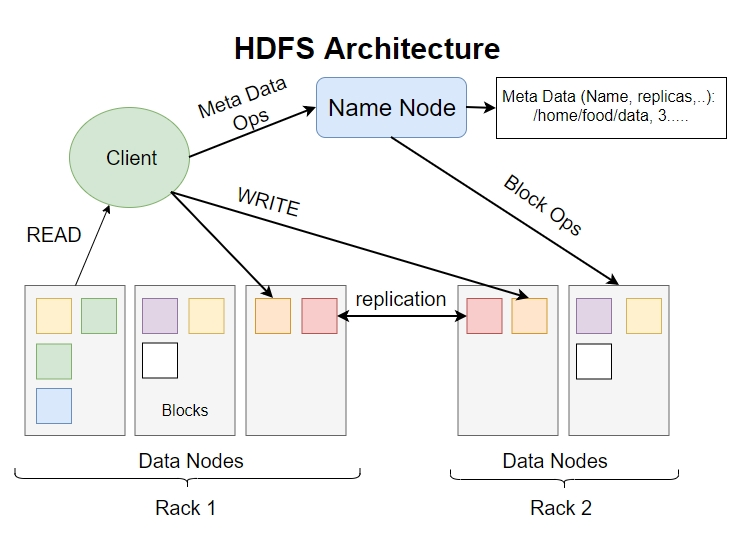
\includegraphics[scale=0.6]{hdfs}  
    \caption[Gambar Hadoop Distributed File System]{Gambar Hadoop Distributed File System} 
    \label{fig:hdfs} 
\end{figure}


HDFS dirancang untuk menyimpan file yang berukuran sangat besar di seluruh mesin dalam {\it cluster} yang besar. HDFS menyimpan setiap file sebagai blok yang berurutan. semua blok dalam file kecuali blok terakhir memiliki ukuran yang sama. Bisa dilihat pada (Gambar ~\ref{fig:hdfs}) bahwa blok-blok file direplikasi untuk memiliki {\it fault tolerance} yang tinggi. Ukuran blok dan banyaknya replika dapat dikonfigurasi untuk setiap file. Faktor replikasi dapat ditentukan pada waktu pembuatan file dan dapat diubah nantinya. File dalam HDFS ditulis sekali dan hanya memiliki satu penulis setiap saat.\\

Namenode mengelola \textit{file system namespaces}. Tidak hanya itu, tugas lain yang dimiliki NameNode adalah memelihara \textit{file system tree} dan metadata untuk semua file dan direktori di pohon. NameNode membuat semua keputusan terkait replikasi blok. NameNode secara berkala menerima Heartbeat dan Blockreport dari masing-masing DataNode di {\it cluster}. Heartbeat mengimplikasikan bahwa DataNode berfungsi dengan benar. Blockreport berisi daftar semua blok pada DataNode. DataNode merupkan pekerja dari sistem file Hadoop. DataNode menyimpan dan mengambil blok ketika diperintahkan oleh NameNode. Selain itu, DataNode melaporkan daftar blok-blok yang disimpan kepada NameNode secara rutin.		
		
		
		\item \textbf{Melakukan studei literatur mengenai Spark)}\\
		{\bf Status :} Ada sejak rencana kerja skripsi \\
		{\bf Hasil :} 
		
\textbf{Pembahasan Umum Spark}

Apache spark adalah sebuah {\it cluster computing platform} dirancang untuk kecepatan dan {\it general-purpose}. Spark dirancang bedasarkan model MapReduce yang populer untuk memberikan dukungan yang efisien kepada banyak tipe komputasi, termasuk {\it interactive query}, dan {\it stream processing} ~\cite{holdenkarau:02:ls}. Kecepatan merupakan kunci dalam memproses data set yang besar, perbedaan waktu dalam eksplorasi data bisa dari beberapa menit sampai beberapa jam tergantung pada kecepatan. Salah satu fitur utama Spark yang ditawarkan adalah kemmapuannya untuk melakukan {\it in memory computations}. Selain itu, sistem Spark lebih efisien daripada MapReduce dalam menjalankan applikasi yang rumit pada disk.\\


Pada sisi {\it general-purpose}, Spark dirancang untuk mencakup berbagai beban kerja yang sebelumnya diperlukan sistem terdistribusi terpisah, termasuk aplikasi \textit{batch}, {\it iterative algorithms}, {\it interactive query}, dan \textit{streaming}. Dengan mendukung beban kerja tersebut di mesin yang sama, Spark membuat pekerjaan lebih mudah dan murah untuk menggabungkan pemrosesan yang berbeda jenis. Dengan begitu, Spark mengurangi beban dalam {\it maintaining} tools-tools yang terpisah.

Spark di desain agar sangat {\it accessible} dengan memberikan API sederhana untuk Python, Java, Scala, dan SQL. Spark denganmudah berintegrasi dengan tools {\it Big Data} lainnya, terutama Hadoop. Spark bisa berjalan dalam Hadoop {\it cluster} dan mengakses sumber data Hadoop mana saja.


\textbf{Komponen Spark}


Proyek Spark memiliki beberapa komponen yang terintegrasi dengan erat. Sebagai {\it core}, Spark adalah "mesin komputasi" yang bertanggung jawab untuk penjadwalan, distribusi, dan pemantauan aplikasi yang terdiri dari banyak {\it computational task} tersebar di banyak pekerja, mesin, atau {\it computing cluster}. Karena {\it core engine} dari Spark cepat dan {\it general-purpose}, Spark menjalankan banyak {\it higer-level components} untuk menangani berbagai macam pekerjaan khuses seprti SQL atau {\it machine learning}. Komponen-komponen ini dirancang untuk saling beroperrasi dengan erat, Spark membiarkan Anda menggabungkan komponen seperti {\it library} dalam suatu proyek perangkat lunak.\\

\begin{figure}[H]
    \centering  
    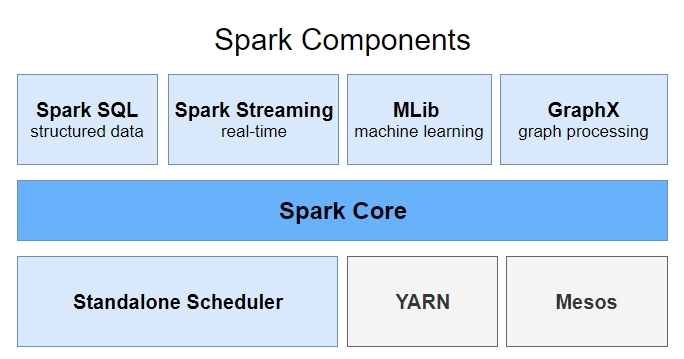
\includegraphics[scale=0.62]{sparkcomponent}  
    \caption[Gambar komponen pada Spark]{Gambar komponen pada Spark} 
    \label{fig:sparkcomponent} 
\end{figure}

Bedasarkan (Gambar ~\ref{fig:hdfs}), Spark memiliki beberapa komponen sebagai berikut:

\begin{itemize}

\item Spark Core:
Spark Core berisi fungsi-fungsi dasar Spark, termasuk komponen untuk tugas penjadwalan, manajemen memori, pemulihan kesalahan, berinteraksi dengan sistem penyimpanan,
dan banyak lagi. Spark Core merupakan rumah bagi API \textit{resilient distributed datasets}(RDD), yang merupakan abstraksi pemrograman utama Spark. RDD mewakili suatu
koleksi \textit{item} yang didistribusikan di banyak node komputasi yang dapat dimanipulasi
secara parallel. Spark Core menyediakan banyak API untuk membangun dan memanipulasi ini
koleksi. 

\item Spark SQL: Spark SQL adalah sebuah \textit{package} untuk bekerja dengan data yang terstuktur. \textit{Package} ini memungkinkan melakukan kueri pada data terstrukut melalui SQL serta varian Apache Hive dari SQL disebut Hive Query Language (HQL) dan \textit{pacakage} ini mendukung banyak sumber data, termasuk tabel Hive, Parket, dan JSON. Selain menyediakan antarmuka SQL untuk Spark, Spark SQL memungkinkan \textit{developer} untuk memadukan kueri SQL dengan manipulasi data terprogram yang didukung oleh RDD pada Python, Java, dan Scala, semua dalam satu aplikasi, sehingga menggabungkan SQL dengan analitik yang rumit. Integrasi ketat dengan lingkungan komputasi yang kaya disediakan oleh Spark membuat Spark SQL tidak seperti gudang data open source lainnya.

\item Spark Streaming: Spark Streaming adalah komponen Spark yang memungkinkan pemrosesan data dari \textit{live streaming}. Contoh \textit{data steam} termasuk file log yang dihasilkan oleh server web produksi, atau antrian pesan yang berisi pembaruan status yang diposting oleh pengguna layanan web. Spark Streaming menyediakan API yang mirip dengan  Spark Core’s RDD API untuk memanipulasi aliran data. Hal ini membuat \textit{developer} mudah memplajari proyek dan berpindah antar aplikasi yang memanipulasi data yang disimpan dalam memori, pada disk, atau tiba dalam \textit{real time}. Di balik API-nya, Spark Streaming dirancang untuk menyediakan tingkat toleransi kesalahan, throughput, dan skalabilitas yang sama seperti Spark Core.

\item MLlib: Spark hadir dengan \textit{library} yang berisi fungsi pembelajaran mesin secara umum (ML), \textit{library} ini disebut MLlib. MLlib menyediakan beberapa jenis algoritma pembelajaran mesin, termasuk klasifikasi, regresi, pengelompokan, dan penyaringan kolaboratif, serta pendukung
fungsionalitas seperti \textit{model evaluation} dan \textit{data import}. MLlib juga menyediakan
beberapa \textit{lower-level} ML \textit{primitives}, termasuk \textit{generic gradient descent optimization
algorithm}.

\item GraphX: GraphX adalah sebuah \textit{library} untuk memanipulasi grafik dan melakukan \textit{graph-parallel computations}. Seperti Spark Streaming dan Spark SQL, GraphX ​​memperluas API Spark RDD, memungkinkan kita untuk membuat \textit{directed graph} dengan\textit{ arbitrary propertiesi} yang melekat pada setiap \textit{vertex} dan \textit{edge}. GraphX ​​juga menyediakan berbagai operator untuk memanipulasi grafik dan memiliki library yang penuh dengan \textit{graph algorithms} yang umum seperti PageRank dan \textit{triangle counting}.

\item Cluster Managers: Spark dirancang untuk \textit{scale up} secara efisien dari satu hingga ribuan node komputasi. Untuk mencapai hal ini dan memaksimalkan fleksibilitas, Spark dapat menjalankan lebih dari satu variasi manajer klaster seperti Hadoop YARN, Apache Mesos, \textit{simple
cluster manager} pada diri Spark sendiri yang disebut \textit{Standalone Scheduler}.

\end{itemize}

\textbf{Tiga Cara Membangun Spark di Atas Hadoop}

\begin{figure}[H]
    \centering  
    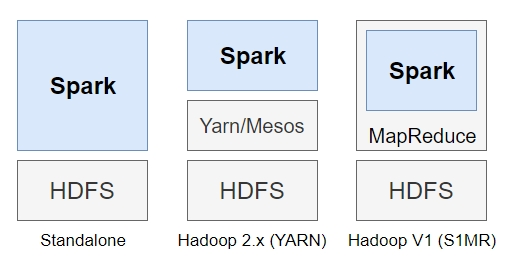
\includegraphics[scale=0.6]{sparkins}  
    \caption[Gambar beberapa cara instalasi Spark]{Gambar beberapa cara instalasi Spark} 
    \label{fig:sparkins} 
\end{figure}

Ada tiga cara untuk meinstalasi Spark bedasarkan (Gambar ~\ref{fig:sparkins}) diatas, ketiga cara tersebut akan dijelaskan dibawah:

\begin{itemize}

\item \textit{Standalone}: Spark \textit{standalone} berarti Spark menempati tempat di atas HDFS (Hadoop Distributed File System) dan ruang dialokasikan untuk HDFS, secara eksplisit. Di sini, Spark dan MapReduce akan berjalan berdampingan untuk mencakup semua pekerjaan percikan di cluster.

\item Hadoop Yarn: Spark berjalan pada Yarn tanpa perlu pra-instalasi atau akses root. Cara ini membantu mengintegrasikan Spark ke dalam ekosistem Hadoop atau Hadoop stack. Cara ini memungkinkan komponen lain untuk berjalan di atas tumpukan.

\item Spark pada MapReduce: Spark pada MapReduce digunakan untuk menjalankan job-job pada spark selain untuk \textit{standalone deployment}. Dengan adanya SIMR, pengguna dapat memulai Spark dan menggunakan \textit{Spark Shell} tanpa akses administratif.

\end{itemize}

\textbf{Resilient Distributed Datasets (RDD)}

Resilient Distributed Datasets (RDD)adalah struktur data dasar Spark. RDD adalah koleksi benda-benda yang didistribusikan secara permanen. Setiap dataset dalam RDD dibagi menjadi beberapa partisi yang dapat dikomputasi pada node yang berbeda pada \textit{cluster} ~\cite{holdenkarau:02:ls}. RDD dapat berisi jenis objek Python, Java, atau Scala, termasuk kelas yang ditentukan pengguna. Spark memanfaatkan konsep RDD untuk mencapai operasi MapReduce yang lebih cepat dan efisien. \\

Secara umun, RDD adalah kumpulan \textit{read-only, partitioned collection} dari \textit{records}. RDD dapat dibuat melalui operasi deterministik dari data pada penyimpanan yang stabil atau RDD lainnya. RDD adalah kumpulan elemen \textit{fault tolerance} yang dapat dioperasikan secara paralel.\\


\textit{Data sharing} pada MapReduce lebih lambat dibanding RDD  karena replikasi, serialisasi, dan disk IO. Sebagian besar aplikasi Hadoop menghabiskan lebih dari 90 persen waktunya untuk melakukan operasi \textit{read-write} keapda HDFS.\\

Untuk menangani masalah tersebut, dibuatlah \textit{framework} khusus disebut Apache Spark. Ide utama dari Spark adalah RDD, Spark mendukung \textit{in-memory computation}. Spark menyimpan status memori sebagai objek di seluruh pekerjaan dan objek dapat dibagi diantara \textit{jobs}. \textit{Data sharing} dalam memori lebih cepat 10 hingga 100 kali lipat dibanding \textit{network} atau \textit{disk}.\\

Berikut adalah sifat-sifat dari RDD :
\begin{itemize}

\item \textit{In Memory}: RDD merupakan sebuah kumpulan object yang berada pada memori. Meskipun
RDD memiliki pilihan untuk disimpan di memori, hardisk, atau bahkan keduanya, kecepatan
eksekusi Spark berdasarkan fakta bahwa data berada dalam memori. Bukan mengambil dari
hard disk setiap kali menjalankan operasi.

\item \textit{Partitioned}: RDD melakukan partisi adalah suatu syarat mutlak teknik untuk mengoptimalkan
performa pada distributed system. Hal ini bertujuan meminimalisir network traffic dan
sekaligus pemungkas high performance workloads. Dalam melakukan partisi, data yang
berupa key/value ditempatkan sesuai dengan rentang key yang bernilai sama. Tujuannya
untuk meminimalisir data yang berpindah-pindah.

\item \textit{Typed}: Data didalam RDD akan selalu digolongkan berdasarkan tipe data.

\item \textit{Lazy evaluation}: \textit{Transformation} pada Spark bersifat ”lazy” atau malas. Ini artinya data didalam RDD tidak akan tersedia sampai dilakukan sebuah action.

\item \textit{Immutable}: RDD yang telah dibuat tidak dapat berubah. Meskipun demikian, RDD
dapat ditransformasi menjadi sebuah RDD baru dengan melakukan perintah \textit{transformation}
pada RDD.

\item \textit{Parallel}: RDD dapat dioperasikan secara pararel.

\item \textit{Cacheable}: Karena RDD bersifat \textit{lazy evaluation}, setiap action yang dilakukan pada RDD akan
menyebabkan RDD mengevaluasi kembali transformasi yang menyebabkan pembuatan RDD. Karena hal ini merupakan sifat yang berdampak buruk pada dataset berukuran besar, maka Spark memberikan pilihan untuk melakukan cache data di memory ataupun pada hard disk.

\end{itemize}

Ada dua cara untuk membuat sebuah RDD. Cara pertama adalah dengan memuat dataset eksternal. Sedangkan cara alternatif adalah dengan mendistribustikan sebuah koleksi objek seperti \textit{list} atau \textit{set}. Ketika sebuah RDD telah dibuat, ada dua tipe operasi yaitu \textit{transformations} dan \textit{actions}. \textit{Transformations} membuat RDD baru dari RDD sebelumnya. Berbeda dengan \textit{tranformations}, \textit{actions} mengembalikan nilai hasil komputasi bedasarkan RDD. Hasil dari \textit{actions} akan dikembalikan kepada \textit{driver program} atau di simpan pada penyimpanan eksternal seperti HDFS.

\begin{verbatim}
//Contoh code membuat RDD dari sumber eksternal 
val lines = sc.textFile("/path/to/README.md")

//Contoh memparalelkan sebuah koleksi pada driver program
val lines = sc.parallelize(["pandas", "ilikepandas"])
\end{verbatim}


\textit{Transformations} pada RDD adalah sebuah operasi yang menerima RDD sebagi masukan dan mengembalikan satu atau lebih RDD baru. RDD masukan tidak berubah karena sifat RDD adalah \textit{immutable} yang berarti tidak bisa diubah ketika dibuat. \textit{Transformations} bersifat \textit{lazy}, \textit{transformation} tidak langsung dieksekusi, melainkan Spark akan mencatat \textit{tranfomartion} apa saja yang dilakukan pada RDD awal. \textit{Transformations} akan dieksekusi ketika sebuah \textit{actions} dipanggil.\\

Berikut adalah contoh filter() transformation di Scala:

\begin{verbatim}
val inputRDD = sc.textFile("log.txt") 
val errorsRDD = inputRDD.filter(line => line.contains("error"))
\end{verbatim}



Berikut adalah Tabel~\ref{tab:trans} berisi daftar \textit{transformations} yang umum pada Spark:

\begin{table}[H] 
	\centering 
	\caption{Tabel transformastions}
	\label{tab:trans}
	\begin{tabular}{ p{6cm}p{9cm}}

\hline
		 \textbf{\textit{Transformations}} & Penjelasan \\
\hline


\hline
\textbf{map}(func) & Mengembalikan dataset terdistribusi baru yang dibentuk dengan melewatkan setiap elemen melalui fungsi func. \\
\hline

\textbf{filter}(func) & Mengembalikan dataset baru yang dibentuk dengan memilih elemen-elemen yang mengembalikan nilai true dari fungsi func. \\
\hline

\textbf{flatMap}(func) & Mirip dengan \textit{map}, tetapi setiap \textit{item input} dapat dipetakan ke nol atau lebih \textit{item output}. \\
\hline
		
\textbf{mapPartitions}(func) & Mirip dengan \textit{map}, tetapi berjalan secara terpisah pada setiap partisi (blok) dari RDD, jadi func harus bertipe Iterator <T> => Iterator <U> ketika menjalankan pada RDD tipe T \\
\hline

\textbf{mapPartitionsWithIndex}(func) & Mirip dengan mapPartitions, tetapi harus menyediakan func dengan nilai integer yang mewakili indeks partisi, jadi func harus bertipe (Int, Iterator <T>) => Iterator <U> ketika menjalankan pada RDD tipe T.\\
\hline

\textbf{sample}(withReplacement, fraction, seed) & 
Mengambil sebagian data sebagai data dengan atau tanpa penggantian menggunakan \textit{random number generator seed} yang diberikan.\\
\hline

\textbf{union}(otherDataset) & Mengembalikan \textit{dataset} baru yang mengandung \textit{element} dari sumber dan \textit{dataset}lainnya.\\

\hline
\textbf{intersection}(otherDataset) & Mengembalikan \textit{dataset} baru yang berisi potongan \textit{element} dari sumber dan \textit{argument}.\\ 

\hline
\textbf{distinct}([numPartitions]) & Mengembalikan \textit{dataset} baru yang mengandung \textit{element} yang unik dari \textit{dataset} sumber.\\

\hline
\textbf{groupByKey}([numPartitions]) & Mengembalikan \textit{dataset} baru bertipe \textit{pairs}  (K, Iterable<V>) dari sumber \textit{dataset} bertipe (K, V).\\


\hline
\textbf{groupByKey}(func,[numPartitions]) & Mengembalikan \textit{dataset} baru bertipe \textit{pairs}  (K, V) yang sudah diagregasi bedasarkan \textit{key} dan \textit{reduce function} yang diberikan.\\

\hline
\textbf{sortByKey}([ascending], [numPartitions]) & Mengembalikan \textit{dataset} baru berupa \textit{pairs}  (K, V) yang terurut secara menaik atau menurun badsarkan parameter boolean yang diberikan.\\

\hline
\textbf{join}(otherDataset, [numPartitions]) & Mengembalikan gabungan \textit{dataset} berupa \textit{pairs}  (K, V) dan (K, W) menjadi \textit{pairs} (K, (V,W)).\\

\hline
\textbf{cogroup}(otherDataset, [numPartitions]) & Mengembalikan \textit{dataset} berupa \textit{tuples}  (K, (Iterable<V>, Iterable<W>)) dari \textit{pairs} (K, V) dan (K, W).\\

\hline
\textbf{cartesian}(otherDataset) & Mengembalikan \textit{dataset} berupa \textit{paris}  (T, U) dari \textit{dataset} T dan U.\\

\hline



	\end{tabular} 
\end{table}

Berikut adalah contoh operasi RDD:
\begin{verbatim}
val lines = sc.textFile("data.txt") 
val pairs = lines.map(s => (s, 1))
val counts = pairs.reduceByKey((a, b) => a + b)
\end{verbatim}

\textit{Actions} merupakah operasi yang mengembalikan sebuah nilai kepada \textit{driver program} atau tempat penyimpanan eksternal. Untuk mengembalikan sebuah nilai, kita bisa menggunakan take(), count(), collect(), dan \textit{actions} lainya. Operasi take() digunakan untuk mengambil sebagian kecil \textit{element} pada RDD. Ketika menggunakan collect(), memori pada satu komputer harus cukup untuk menampung seluruh \textit{dataset}. Operasi tersebut baiknya digunakan pada \textit{dataset} yang berukuran kecil dan \textit{dataset} berukuran besar bisa disimpan pada tempat penyimpanan eksternal. Setiap kali \textit{actions} baru dipanggil, seluruh RDD akan dikomputasi dari akarnya. Untuk mencapai efisiensi yang lebih tinggi, bisa dilakukan \textit{persist} terhadap \textit{intermediate
results}. \\

Berikut adalah Tabel~\ref{tab:actions} berisi daftar \textit{actions} yang umum pada Spark:


\begin{table}[H] 
	\centering 
	\caption{Tabel Actions}
	\label{tab:actions}
	\begin{tabular}{p{6cm}p{9cm}	}

\hline
		 \textbf{\textit{Actions}} & Penjelasan \\
\hline


\hline
\textbf{reduce}(func) & Mengagregasikan seluruh \textit{element} pada \textit{dataset} menggunakan fungsi yang diberikan pada \textit{parameter}. \\

\hline
\textbf{collect}() & Mengembalikan seluruh \textit{dataset} sebagai array kepada \textit{driver program}. \\

\hline
\textbf{count}() & Mengembalikan jumlah \textit{element} pada \textit{dataset}. \\

\hline
\textbf{first}() & Mengembalikan \textit{element} pertama pada \textit{dataset}. \\

\hline
\textbf{take}(n) & Mengembalikan sebuah array dengan n jumlah \textit{element} pertama dari \textit{dataset}.\\

\hline
\textbf{takeSample}(withReplacement, x, [seed]) & Mengembalikan sebuah array dengan x jumlah \textit{element} secara acak dari \textit{dataset}. \\

\hline
\textbf{takeOrdered}(n, [ordering]) & Mengembalikan sebuah array dengan n jumlah \textit{element} pertama dari \textit{dataset} secara terurut. \\

\hline
\textbf{saveAsTextFile}(path) & Menyimpan \textit{dataset} sebagai \textit{text file} pada direktori yang ditentukan. \\

\hline
\textbf{saveAsSequenceFile}(path) & Menyimpan \textit{dataset} sebagai Hadoop SequenceFile pada direktori yang ditentukan.\\

\hline
\textbf{saveAsObjectFile}(path) & Menyimpan \textit{dataset} sebagai format yang sederhana menggunakan Java Serialization pada direktori yang ditentukan.\\

\hline
\textbf{countByKey}() & Menjumlahkan \textit{pairs} (K, V) bedasarkan \textit{key} dan mengembalikan sebuah \textit{pairs} berisi (K, int). \\

\hline
\textbf{foreach}(func) & Memproses setiap \textit{element} pada \textit{dataset} menggunakan fungsi func yang diberikan. \\

\hline



	\end{tabular} 
\end{table}
		
		
		
		\item \textbf{Melakukan studi literatur mengenai bahasa pemrograman Scala}\\
		{\bf Status :} Ada sejak rencana kerja skripsi \\
		{\bf Hasil :} Scala adalah sebuah bahasa pemrograman yang diciptakan oleh Martin Odersky yaitu seorang Profesor di Ecole Polytechnique Federale de Lausanne, sebuah kampus di Lausanne, Swiss. Kata Scala sendiri merupakan kependekan dari “Scalable Language”. Karena Scala berjalan diatas Java Virtual Machine (JVM), Scala memiliki performa yang relatif cepat dan juga memungkinkan untuk menggabungkan kode di Scala dengan di Java. Termasuk library, framework dan tool yang ada di Java, bisa gunakan di Scala. Scala menggabungkan konsep Object Oriented Programming (OOP) yang dikenal di Java dengan konsep Functional Programming (FP). Adanya konsep FP inilah yang menjadikan Scala sangat ekspresif, nyaman dan menyenangkan untuk digunakan. \\

Perintah $’scalac’$ digunakan untuk mengkompilasi program Scala dan akan menghasilkan beberapa file kelas di direktori saat ini. Salah satunya akan disebut file .class. Ini adalah bytecode yang akan berjalan di Java Virtual Machine (JVM) dengan menggunakan perintah $’scala’$. \\

\textbf{Expressions}

suatu \textit{ekspressions} adalah pernyataan atau argumen yang dapat dikomputasi.\\

\begin{verbatim}
1 + 1
2 + 2
\end{verbatim}


\textit{Ekspressions} dapat dikembalikan dengan perintah println.

\begin{verbatim}
println(1)
println(100) // 100
println(1 + 1) // 2
println("Hi!") // Hi!
\end{verbatim}


\textit{Ekspressions} atau pernyataan seperti diatas dapat disimpan dalam sebuah variable ada dua jenis variable di Scala yaitu val dan var. Setelah val diinisialisasi, val tidak dapat diisi kembali artinya isi dari val tidak dapat diubah.

\begin{verbatim}
val x = 2 + 5
val x = 10 //tidak akan di compile 
val y = 7
val coba:Int = 200 
\end{verbatim}

variable mirip dengan value, tetapi nilai variable bisa di isi kembali.

\begin{verbatim}
var x = 2 + 2 
x = 4 
println(x) // 4 
x = 7 
println(x) // 7 
\end{verbatim}

Secara eksplisit kita bisa menyatakan tipe dari sebuah var atau val dengan cara:

\begin{verbatim}
var x: Int = 1 + 1 // Int merupakan tipe dari variable x
val y: Long = 987654321 // Long merupakan tipe dari variable y
val z: Char = 'a' // Char merupakan tipe dari variable z
\end{verbatim}

\textbf{Blocks}

Block digunakan untuk menggabungkan \textit{expressions}. Berikut adalah contoh \textit{block}:

\begin{verbatim}
println({
    val x = 1 + 1
    x + 1
}) // 3 
\end{verbatim}

\textbf{Loop dan Conditional}

loop adalah struktur pengulangan yang memungkinkan untuk menulis secara efisien suatu loop yang perlu dieksekusi sejumlah kali. Ada berbagai bentuk loop dalam Scala yang dijelaskan di bawah ini: 

\begin{verbatim}
for( var x <- Range ){
    statement(s);
}

var x = 0
while (x < 10) {
    println(x)
    i += 1
}
\end{verbatim}

Percabangan adalah pengujian sebuah kondisi. Jika kondisi yang diuji tersebut terpenuhi, maka program akan menjalankan pernyataan-pernyataan tertentu. Jika kondisi yang diuji salah, program akan menjalankan pernyataan yang lain. Berikut adalah contoh percabangan dalam bahasa Scala:

\begin{verbatim}
if( x < 20 ){
    println("This is if statement");
}

if( x < 20 ){
    if( x< 5) {
        println("smallest");
    }
}

if( x < 10 ){
    println("This is bigger");
} else { 
    println("This is smaller");
}

if( x == 1 ){
    println("1");
} else if (x == 2){ 
    println("2");
}
\end{verbatim}


\textbf{Functions}

\textit{Functions} adalah \textit{expression} yang mempunyai atau menerima parameter. Sebuah function yang tidak memliki nama disebut anonymous function. Berikut adalah contoh anonymous function dan function biasa. Sebuah function bisa memiliki lebih dari satu parameter.

\begin{verbatim}
(x: Int) = > x + 1 // Anonymous function 

val addOne = (x: Int) => x + 1 // function biasa 
println(addOne(2)) // 3 

val add = (x: Int, y: Int) => x + y 
println(add(1, 2)) // 3 
\end{verbatim}

Pada sisi sebelah kiri tanda => adalah parameter-parameter sebuah function, pada sisi kanan merupakan expresi-expresi yang melibatkan parameter tersebut. \\


\textbf{Methods}

Method hampir sama dengan functionn, tetapi method memiliki beberapa perbedaan. Method harus di definisikan dengan kata kunci def, diikuti dengan nama method, paramter-parameter dari method tersebut, tipe kembalian method, dan \textit{body dari method tersebut}. 

\begin{verbatim}
def add(x: Int, y: Int): Int = x + y 
println(add(1, 2)) // 3 
\end{verbatim}

Method bisa mempunyai lebih dari satu parameter \textit{list} 

\begin{verbatim}
def addThenMultiply(x: Int, y: Int)(multiplier: Int): Int = (x + y) * multiplier 
println(addThenMultiply(1, 2)(3)) // 9 
\end{verbatim}


Method yang tidak memiliki parameter

\begin{verbatim}
def name: String = System.getProperty("user.name")
println("Hello, " + name + "!")
\end{verbatim}
Method berbeda dengan functions bisa memiliki \textit{multi-line expressions}

\begin{verbatim}
def getSquareString(input: Double): String = {
    val square = input * input
    square.toString
}
\end{verbatim}

Expresi terakhir dari method menjadi nilai yang akan dikembalikan. Scale memunyai \textit{keyword} return, tetapi sangat jarang digunakan.\\

\textbf{Class dan Object}

Class pada Scala di definisikan dengan kata kunci class diikuti dengan namanya dan terakhir adalah consturctor parameter.

\begin{verbatim}
class Greeter(prefix: String, suffix: String) {
    def greet(name: String): Unit = {
        println(prefix + name + suffix)
    }
}
\end{verbatim}



Dibawah adalah cara mendeklarasi objek dan pemanggilan method pada Scala 

\begin{verbatim}
val greeter = new Greeter("Hello, ", "!")
greeter.greet("Scala developer")
\end{verbatim}

Objek dapat dianggap sebagai sesuatu instansi yang tunggal pada class itu sendiri. Untuk mendefinisikan objek, digunakan kata kunci Object. 

\begin{verbatim}
object IdFactory {
    private var counter = 0
  
    def create(): Int = {
      counter += 1
      counter
    }
}

val newId: Int = IdFactory.create()
println(newId) // 1
val newerId: Int = IdFactory.create()
println(newerId) // 2
\end{verbatim}

Main method adalah sebuah pintu masuk dari sebuah program. Java Virtual Machine membutuhkan sebuah main method yang dinamakan main dan menerima satu argument, seubah array bertipe string.\\

Menggunakan \textit{object}, kita bisa mendefinisikan sebuah main method seperti berikut: 

\begin{verbatim}
object Main {
    def main(args: Array[String]): Unit = {
        println("Hello, Scala developer!")
    }
}
\end{verbatim}

\textbf{Higher Order Function}

Pada bahasa Scala ada yang disebut sebagai Higher Order Function. Higher Order Function merupakan sebuah function yang menerima function lainya sebagai parameter dan mengembalikan sebuah function sebagai hasilnya. Berikut adalah contoh-contoh Higher Order Function:

\begin{verbatim}
val salaries = Seq(20000, 70000, 40000)
val doubleSalary = (x: Int) => x * 2
val newSalaries = salaries.map(doubleSalary) // List(40000, 140000, 80000)
\end{verbatim}

Kita bisa mempersingkat kode dengan sebuah function anonymous dan langsung dimasukan pada parameter

\begin{verbatim}
val salaries = Seq(20000, 70000, 40000)
val newSalaries = salaries.map(x => x * 2) // List(40000, 140000, 80000)
\end{verbatim}

Kita juga dapat memasukan method pada parameter higher order function, compiler Scala akan mengubah sebuah method menjadi function.


\begin{verbatim}
case class WeeklyWeatherForecast(temperatures: Seq[Double]) {

    private def convertCtoF(temp: Double) = temp * 1.8 + 32 // sebuah method

    def forecastInFahrenheit: Seq[Double] = temperatures.map(convertCtoF) } 
    // method sebagai parameter
}
\end{verbatim}


Salah satu alasan untuk menggunakan higher order function adalah untuk mengurangi kode yang berlebihan. Katakanlah ada beberapa metode yang dapat menaikkan gaji seseorang dengan berbagai faktor. Tanpa membuat fungsi urutan tinggi, mungkin terlihat seperti ini:

\begin{verbatim}
object SalaryRaiser {

    def smallPromotion(salaries: List[Double]): List[Double] =
      salaries.map(salary => salary * 1.1)

    def greatPromotion(salaries: List[Double]): List[Double] =
      salaries.map(salary => salary * math.log(salary))

    def hugePromotion(salaries: List[Double]): List[Double] =
      salaries.map(salary => salary * salary)
}
\end{verbatim}

Perhatikan bahwa masing-masing dari ketiga method hanya berbeda pada faktor perkalian. Untuk menyederhanakan, kita dapat mengeluarkan kode yang redundan menjadi higher order function seperti:


\begin{verbatim}
object SalaryRaiser {

    //Higher Order Function
    private def promotion(sal: List[Double], func: Double => Double): List[Double] =
      salaries.map(func)  

    def smallPromotion(sal: List[Double]): List[Double] =
      promotion(sal, salary => salary * 1.1)

    def bigPromotion(sal: List[Double]): List[Double] =
      promotion(sal, salary => salary * math.log(salary))

    def hugePromotion(sal: List[Double]): List[Double] =
      promotion(sal, salary => salary * salary)
}
\end{verbatim} 
	
	\item \textbf{Melakukan studi literatur mengenai teknik-teknik reduksi data dan algoritma agglomerative}\\
		{\bf Status :} Ada sejak rencana kerja skripsi \\
		{\bf Hasil :} Meledaknya ukuran data, jumlag \textit{record}, dan attribut data membuat pengenbangan baru dalam teknik mereduksi data.  Mereduksi data merupakan bagian penting dalam bidang \textit{big data}. Data direkduksi agar lebih mudah diolah dan diterapkan teknik-teknik \textit{data mining}. Teknik yang digunakan dalam mereduksi data sangat tergantung dengan tipe data yang ditangani dan tujuan akhir dalam mereduksi data. Dalam mereduksi data, data yang direduksi harus bisa mewakili data metah secara keseluruhan. Bila data yang sudah direduksi tidak mewakili data awal, tidak ada gunanya untuk mereduksi data.\\
		
Berikut adalah contoh dan penjelasan beberapa teknik:

\begin{itemize}

\item \textit{Missing Values Ratio}: Kolom data dengan nilai yang terlalu banyak hilang kemungkinan tidak akan membawa banyak informasi yang berguna. Kolom data dengan jumlah nilai yang hilang lebih besar dari batas yang diberikan dapat dihapus. Semakin tinggi batas, semakin agresif pengurangannya.

\item \textit{Low Variance Filter}: Mirip dengan teknik sebelumnya, kolom data dengan sedikit perubahan dalam data membawa sedikit informasi. Jadi semua kolom data dengan varians lebih rendah dari batas yang diberikan akan dihapus. Normalisasi diperlukan sebelum menerapkan teknik ini.

\item \textit{High Correlation Filter}: kolom data dengan kecenderungan yang sangat mirip biasanya membawa informasi yang sangat mirip. Dalam hal ini, hanya satu saja yang cukup untuk diberikan kepada model pembelajaran mesin. Di sini kita menghitung koefisien korelasi antara kolom numerik dan antara kolom nominal sebagai Pearson's Product Moment Coefficient dan nilai chi square Pearson masing-masing. Pasangan kolom dengan koefisien korelasi lebih tinggi dari batas digabungkan menjadi hanya satu.

\item \textit{Random Forests / Ensemble Trees}: Algoritma ini digunakan pada klasifikasi data dalam jumlah yang besar. Klasifikasi \textit{random forest} dilakukan melalui penggabungan pohon dengan melakukan \textit{training} pada sampel data yang dimiliki. Penggunaan pohon yang semakin banyak akan mempengaruhi akurasi yang akan didapatkan menjadi lebih baik. Penentuan klasifikasi dengan \textit{random forest} diambil berdasarkan hasil voting dari pohon yang terbentuk. Pemenang dari pohon yang terbentuk ditentukan dengan vote terbanyak. Pembangunan pohon  pada \textit{random forest} sampai dengan mencapai ukuran maksimum dari pohon data. Akan tetapi, pembangunan pohon \textit{random forest} tidak dilakukan  \textit{pruning} yaitu sebuah metode untuk mengurangi kompleksitas ruang. Pembangunan dilakukan dengan penerapan metode seleksi fitur secara acak untuk meminimalisir kesalahan. Pembentukan pohon  dengan sample data menggunakan variable yang diambil secara acak dan menjalankan klasifikasi pada semua tree yang terbentuk. \textit{Random forest} menggunakan \textit{Decision Tree} untuk melakukan proses seleksi. Pohon yang dibangun dibagi secara rekursif dari data pada kelas yang sama. Pemecahan  digunakan untuk membagi data berdasarkan jenis atribut yang digunakan.

\item \textit{Principal Component Analysis (PCA)}: PCA adalah prosedur statistik yang secara ortogonal mengubah koordinat n asli dari satu set data menjadi satu set baru dari n koordinat yang disebut komponen utama. Sebagai hasil dari transformasi, komponen utama pertama memiliki kemungkinan varian terbesar; setiap komponen yang berhasil memiliki kemungkinan varian tertinggi di bawah batasan yang bersifat ortogonal terhadap. PCA menjaga hanya komponen m < n komponen pertama mengurangi dimensi data sambil mempertahankan sebagian besar informasi data, yaitu variasi dalam data.

\item \textit{Backward Feature Elimination}: Pada teknik ini, pada iterasi yang diberikan, algoritma klasifikasi yang dipilih dilatih pada n fitur input. Kemudian, dihapus satu fitur masukan pada satu waktu dan melatih model yang sama pada fitur masukan n-1 kali n. Fitur input yang penghapusannya telah menghasilkan peningkatan terkecil dalam tingkat kesalahan dihapus, meninggalkan kita dengan fitur input n-1. Klasifikasi ini kemudian diulang menggunakan fitur n-2, dan seterusnya. Setiap iterasi k menghasilkan model yang dilatih pada fitur n-k dan tingkat kesalahan e (k). Memilih tingkat kesalahan maksimum yang dapat ditolerir, kami menetapkan jumlah terkecil fitur yang diperlukan untuk mencapai kinerja klasifikasi dengan algoritme pembelajaran mesin yang dipilih.

\item \textit{Forward Feature Construction}: Teknik ini adalah teknik kebalikan dari \textit{Backward Feature Elimination}. Dimulai dari satu fiture, dan secara bertahap ditambahkannya fitur yang menghasilkan kenaikan performa yang paling tinggi. Kedua algoritma memiliki konsumsi waktu dan komputasi yang tinggi. Algoritma tersebut baiknya digunakan pada \textit{data set} dengan colom input yang sedikit.



\end{itemize}
		
\textit{Hierarchical Clustering Algorithm} (HCA) adalah metode analisis kelompok yang berusaha untuk membangun sebuah hirarki dengan mengelompokan data. Dengan mengelompokan data-data tersebut, data pada kelompok yang sama memiliki kemiripan yang tinggi dan data pada kelompok yang berbeda memiliki kemiripan yang rendah. Dalam reduksi data, \textit{cluster} yang merepresentasikan data-data pada \textit{cluster} tersebut akan diggunakan untuk mengganti data-data mentah. Seberapa efektif cara ini tergantung dengan sifat data yang ditangani. Data yang bisa dikelompokan kedalam cluster yang berbeda akan sangat cocok dengan cara ini. Pada dasarnya HCA dibagi menjadi dua jenis yaitu Agglomerative (Bottom-Up) dan Devisive (Top-Down).\\

Agglomeratice hierarchical clustering memulai dengan setiap objek membentuk sub-cluster tersendiri dan secara iterative menggabung sub-cluster menjadi sub-cluster yang lebih besar sampai semua objek berada pada satu cluster. Pada tahap pegabungan, cluster yang terdekat bedasarkan similaritas tertentu akan digabungkan menjadi satu. Pada setiap iterasi akan ada 2 buah cluster yang dibagung menjadi satu, maka dari itu agglomerative clustering akan hanya membutuhkan maksimal n iterasi. Dendogram sangat umum digunakan untuk menggambarkan proses HCA. \\


\begin{figure}[H]
    \centering  
    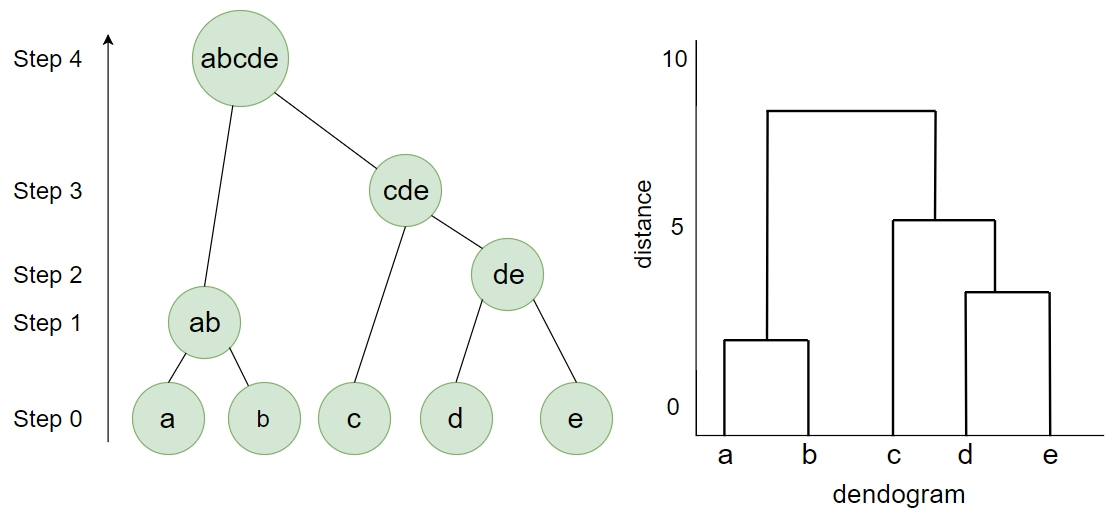
\includegraphics[scale=0.5]{dendo}  
    \caption[Gambar {\it dendogram} ]{Gambar {\it dendogram}} 
    \label{fig:dendo} 
\end{figure}

Berdasakan gambar diatas (Gambar ~\ref{fig:dendo}), berikut adalah langkah-langkah:

\begin{enumerate}

\item Hitung Matrik Jarak antar objek.

\item Gabungkan dua kelompok terdekat berdasarkan parameter kedekatan yang ditentukan.

\item Perbarui Matrik Jarak antar objek untuk merepresentasikan kedekatan diantara kelompok baru dan kelompok yang masih tersisa.

\item Ulangi langkah 2 dan 3 higga hanya satu kelompok yang tersisa.

\end{enumerate}

Berikut adalah tiga metode pengelompokan Agglomerative Hierarchical:

\begin{itemize}

\item Single Linkage (Jarak Terdekat): Sebuah sub-tree atau sub-cluster cp dikelompokan dengan sub-cluster cq menggunakan 
minimum distance antara \textit{object members} pada cp dan cq (edge terdekat)

\begin{verbatim}
dmin = min(dij)
1 <= i <= m 
1 <= j <= n

dij = adalah jarak antara objek i pada cp dan j pada cq; 
m = jumlah objek pada sub-cluster cp
n = jumlah objek pada sub-cluster cg.
\end{verbatim}

\item Complete Linkage (Jarak Terjauh): Sebuah sub-tree atau sub-cluster cp dikelompokan dengan sub-cluster cq menggunakan 
maximum distance antara \textit{object members} pada cp dan cq (edge terjauh)

\begin{verbatim}
dmin = max(dij)
1 <= i <= m 
1 <= j <= n

dij = adalah jarak antara objek i pada cp dan j pada cq; 
m = jumlah objek pada sub-cluster cp
n = jumlah objek pada sub-cluster cg.
\end{verbatim}

\item  Average Linkage (Jarak Rata-Rata): Sebuah sub-tree atau sub-cluster cp dikelompokan dengan sub-cluster cq menggunakan 
average distance antara \textit{centroid ci} dan \textit{centroid cg}.

\begin{verbatim}
dmeans = distance(centroidcp, centroidcq)
centroidcp = jarak rata-rata semua artibute pada sub-cluster Cp 
centroidcp = jarak rata-rata semua artibute pada sub-cluster Cg
\end{verbatim}

\end{itemize}
		
	\item \textbf{Melakukan instalasi Spark dan eksplorasi Spark shell}\\
		{\bf Status :} Ada sejak rencana kerja skripsi \\
		{\bf Hasil :}

Pada bagian ini, akan dijelaskan tahap-tahap untuk melakukan instalasi Apache Spark. Apache Spark yang akan digunakan adalah Apache Spark versi x Spark dapat berjalan diatas berbagai sistem operasi seperti Window Windows dan UNIX systems (Contoh Linux, Mac OS). Sebelum memulai instalasi Apache Spark, ada beberapa kebutuhan yang harus dipenuhi seperti instalasi JAVA dan Scala. Berikut adalah langkah-langkah untuk memastikan kita telah memenuhi kebutuhan minimal:

\begin{itemize}

\item Cek apakah Java telah diinstall dan versi java yang diinstall adalah setidaknya 8+ karena Spark berjalan pada versi minimal Java 8+. Berikut adalah command untuk memastikan java telah terinstall.

\begin{verbatim}
java -version

Java(TM) SE Runtime Environment (build 1.8.0_112-b15)                                                                   Java HotSpot(TM) 64-Bit Server VM (build 25.112-b15, mixed mode) 

\end{verbatim}


\item Jika scala belum di installasi pastikan di install dengan versi minimal 2.11.x. 

\begin{verbatim}

scala -version

Scala code runner version 2.11.6 -- Copyright 2002-2013, LAMP/EPFL

\end{verbatim}

\end{itemize} 

Bila kita tidak memliki JAVA dan Scala pada komputer, berikut adalah cara menginstall JAVA dan Scala untuk kebutuhan Spark:

\begin{itemize}

\item Berikut adalah comand-comand untuk menginstall Java menggunakan terminal pada sistem operasi Linux:

\begin{verbatim}
sudo apt-get update
sudo apt-get install default-jdk
\end{verbatim}

\item Berikut adalah comand-comand untuk menginstall Scala menggunakan terminal pada sistem operasi Linux:

\begin{verbatim}
sudo apt-get update
sudo apt-get install scala
\end{verbatim}

\end{itemize}


Instalasi dapat dilakukan ketika syarat-syarat diatas telah dipenuhi. Berikut adalah langkah-langkah instalsi Apache Spark:

\begin{enumerate}

\item Pertama, donwload versi spark yang diinginkan  dari link https://spark.apache.org/downloads.html

\item Kemudian extract Spark tar dengan command berikut:

\begin{verbatim}
tar xvf spark-2.3.1-bin-hadoop2.7.tgz 

su – 
Password:

cd /home/usr/Downloads/ 
mv spark-2.3.1-bin-hadoop2.7 /usr/local/spark 
exit 

\end{verbatim}

\item Kemudian kita harus menkonfigurasi environment variable untuk Spark. Ubah file .bsshrc dengan menbahkan command berikut pada file.

\begin{verbatim}
export PATH=$PATH:/usr/local/spark/bin
\end{verbatim}

\item Terakhir jalankan command berikut untuk memastikan perubahan telah terjadi pada file ~/.bashrc.

\begin{verbatim}
source ~/.bashrc
\end{verbatim}

\item Ketika spark diinstall dengan benar, maka dengan command spark-shell kita bisa menjalankan spark shell (Gambar~\ref{fig:sparkshell}).

\begin{verbatim}
$ SPARK_HOME/bin/spark-shell
\end{verbatim}

\begin{figure}[H]
    \centering  
    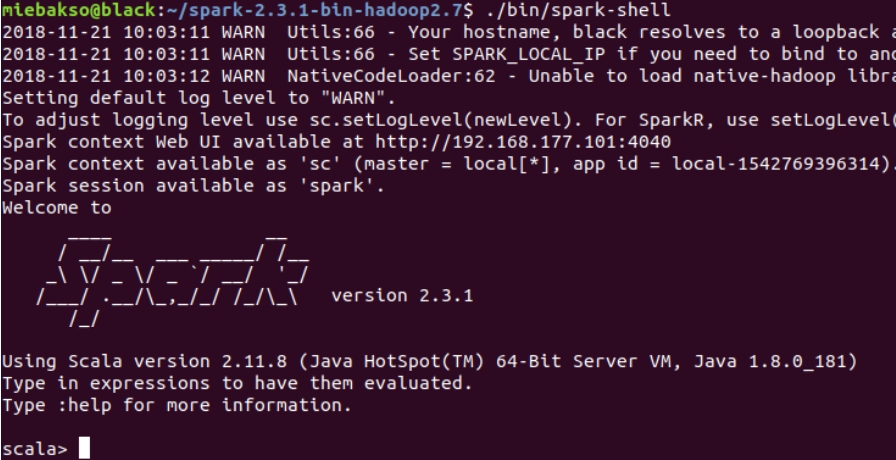
\includegraphics[scale=0.5]{sparkshell}  
    \caption[Gambar {\it Spark Shell} ]{Gambar {\it Spark Shell}} 
    \label{fig:sparkshell} 
\end{figure}

\end{enumerate}


\textbf{Eksplorasi Spark Shell}\\

Pada bagian ini, penulis akan menjelaskan percoba \textit{word count} pada file text README.md. Penulis akan menggunakan Spark Shell untuk menjalankan perintah-perintah agar spark bisa menghitung jumlah setiap kata yang ada pada text file tersebut. Setiap kata yang sama akan dijumlahkan. Pada bagian ini akan digunakan tranformation dan juga action.

\begin{figure}[H]
    \centering  
    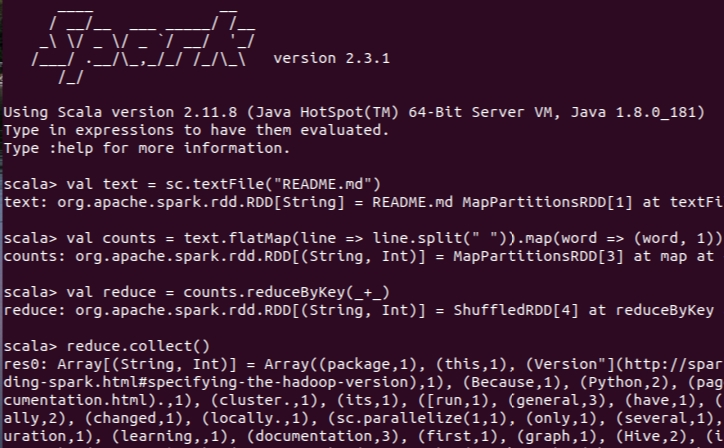
\includegraphics[scale=0.6]{wordcount}  
    \caption[Gambar {\it Word Count} ]{Gambar {\it Word Count}} 
    \label{fig:wordcount} 
\end{figure}

Bedasarkan gambar diatas (Gambar~\ref{fig:wordcount}), berikut adalah langkah-langkah percobaan  \textit{word count}:

\begin{enumerate}

\item Pertama, kita jalankan spark shell dengan command berikut pada terminal.

\begin{verbatim}
$ ./bin/spark-shell
\end{verbatim}

\item Setelah itu, kita akan membuat text RDD dengan megambil sumber eksternal yaitu file README.md. Command dibawah digunakan untuk membuat RDD dari file eksternal.

\begin{verbatim}
val text = sc.textFile("README.md") 
text: org.apache.spark.rdd.RDD[String] = README.md MapPartititonsRDD[1] at textFile at <console>:24
\end{verbatim}

\item Kemudian, kita akan memisahkan setiap kata menjadi pairs dengan kata sebaya key dan 1 sebagi value setiap kata.

\begin{verbatim}
val counts = text.textflatMap(line => line.split(" ")).map(word => (word, 1))
counts: org.apache.spark.rdd.RDD[(String, int)] = ShuffledRDD[3] at map at <console>:25
\end{verbatim}

\item Langkah selanjutnya, kita akan menghitung jumlah setiap kata dengan cara berikut.

\begin{verbatim}
val reduce = counts.reduceByKey(_+_)
reduce: org.apache.spark.rdd.RDD[(String, int)] = ShuffledRDD[4] at reduceByKey at <console>:25
\end{verbatim}

\item Terakhir, kita akan mengambil hasil.

\begin{verbatim}
reduce.collect()
res0: Array[(String, Int)] = Array((package,1), (Python,2), ..... 
\end{verbatim}

\end{enumerate}

\textbf{Instalasi Spark pada multi-node cluster}\\

Pada bagian ini, penulis akan menjelaskan langkah-langkah yang diperlukan untuk menginstall Spark pada multi-node cluster. Berikut adalah langkah-langkah yang harus dilakukan:

\begin{enumerate}

\item Tambahkan entri dalam file host (master dan slave)

\begin{verbatim}
$ sudo vim /etc/hosts

\\tambahkan IP master dan juga slave 

<MASTER-IP> master
<SLAVE1-IP> slave1
<SLAVE2-IP> slave2
<SLAVE3-IP> slave3
\end{verbatim}

\item Kemudian install Java pada setiap master dan slave, jangan lupa cek versi java yang diinstall

\begin{verbatim}
$ sudo apt-get update
$ sudo apt-get install default-jdk

\\Setelah itu cek versi java yang diinstal

$ java -version
\end{verbatim}

\item Kemudian install Scala pada setiap master dan slave, jangan lupa cek versi scala yang diinstall.

\begin{verbatim}
$ sudo apt-get update
$ sudo apt-get install scala

\\Setelah itu cek scala java yang diinstal

$ scala -version
\end{verbatim}

\item Install Open SSH Server-Client pada master.

\begin{verbatim}
\\Untuk install Open SSH
$ sudo apt-get install openssh-server openssh-client

\\Generate key pairs
$ ssh-keygen -t rsa -P ""

Selanjutkna kita perlu konfigurasi SSH pada slave dan juga master. 
Copy .ssh/id_rsa.pub miliki master kepada .ssh/authorized_keys untuk master dan juga slave.
\end{verbatim}



\item Setelah itu, kita akan download dan install Spark pada setiap slave dan master.

\begin{verbatim}
\\Dowload versi spark yang diinginkan pada 
https://spark.apache.org/downloads.html

\\extract spark dengan comand berikut
$ tar xvf spark-2.3.0-bin-hadoop2.7.tgz

\\pindahkan spark kepada direktori yang diinginkan
$ sudo mv spark-2.3.0-bin-hadoop2.7 /direktori/yang/diinginkan/
\end{verbatim}

\item Sesudah download maka kita harus mengubah file bashrc.

\begin{verbatim}
$ sudo vim ~/.bashrc

export PATH = $PATH:/usr/local/spark/bin

$ source ~/.bashrc
\end{verbatim}

\item Kemudian kita harus konfigurasi Spark master dengan mengubah file spark-env.sh.

\begin{verbatim}
$ cd /usr/local/spark/conf
$ cp spark-env.sh.template spark-env.sh

\\Edit spark-env.sh
$ sudo vim spark-env.sh

export SPARK_MASTER_HOST='<MASTER-IP>'
export JAVA_HOME=<Path_of_JAVA_installation>

Kemudian edit file slave pada /usr/local/spark/conf

$ sudo vim slaves

master
slave1
slave2
slave3
\end{verbatim}

\item Sekarang, kita bisa menjalankan spark cluster

\begin{verbatim}
$ cd /usr/local/spark
$ ./sbin/start-all.sh

//Untuk memberhentikan cluster masukan comand berikut
$ ./sbin/start-all.sh
\end{verbatim}


\end{enumerate}


\item \textbf{Merancang sebagian kustomisasi algoritma berbasis spark}\\
		{\bf Status :} Ada sejak rencana kerja skripsi \\
		{\bf Hasil :} Berikut adalah rancangan algoritma kustomisasi yang masih belum sempurna. 

\begin{lstlisting}
object Hello extends App {

	var x:CustomAgglo = new CustomAggloe()
}

class CustomAgglo(var rec: Map[Int,List[Int]], max:Int, var dist:Int, var coff:Int) {

    //create array list
    var treeList = Array.fill[SingleTree](max) 
    //Immutable MASALAH, tidak ada arraylist
    var count:Int
    var isProceed:Boolean

    def customRun(): Unit ={
        count = 0;
        for( x <- rec){
            //Form independent tree from x add x to treeList
			
            isProceed=false
            if(count==max){
                //form dendogram tree using dist type
                //form object cluster using distace measure
                //clear object tree & remove from memory
                isProceed=true
            }
        }
        if(isProceed==false){
            //form dendogram tree using dist type
            //form object cluster using distace measure
            //clear object tree & remove from memory
        }
    }

}

class SingleTree(var attVal: List[Int], var clsLabel:Int){
    var x = 2

}
\end{lstlisting}

		
\end{enumerate}

\section{Pencapaian Rencana Kerja}
Langkah-langkah kerja yang berhasil diselesaikan dalam Skripsi 1 ini adalah sebagai berikut:
\begin{enumerate}
\item Melakukan studi literatur \textit{big data}.
\item Melakukan studi literatur Hadoop.
\item Melakukan studi literatur Spark.
\item Melakukan studi literatur bahasa pemrograman Scala.
\item Melakukan studi literatur algoritma reduksi data dan agglomerative.
\item Membuat rancangan algoritma reduksi data dalam bahasa Scala.
\item Mengerjakan dokumen skripsi sampai bab 4 awal.

\end{enumerate}

\section{Kendala yang Dihadapi}
Kendala - kendala yang dihadapi selama mengerjakan skripsi :
\begin{itemize}
	\item Kesulitan dalam mempelajari bahasa Scala.
	\item Terlalu banyak les bahasa Inggris dan bahasa Jerman.
	\item Komputer lab skripsi ke lock terus menerus kita ingin mencoba dan harus bergantian dengan yang lain.
\end{itemize}

\vspace{1cm}
\centering Bandung, \tanggal\\
\vspace{2cm} \nama \\ 
\vspace{1cm}

Menyetujui, \\
\ifdefstring{\jumpemb}{2}{
\vspace{1.5cm}
\begin{centering} Menyetujui,\\ \end{centering} \vspace{0.75cm}
\begin{minipage}[b]{0.45\linewidth}
% \centering Bandung, \makebox[0.5cm]{\hrulefill}/\makebox[0.5cm]{\hrulefill}/2013 \\
\vspace{2cm} Nama: \pembA \\ Pembimbing Utama
\end{minipage} \hspace{0.5cm}
\begin{minipage}[b]{0.45\linewidth}
% \centering Bandung, \makebox[0.5cm]{\hrulefill}/\makebox[0.5cm]{\hrulefill}/2013\\
\vspace{2cm} Nama: \pemB \\ Pembimbing Pendamping
\end{minipage}
\vspace{0.5cm}
}{
% \centering Bandung, \makebox[0.5cm]{\hrulefill}/\makebox[0.5cm]{\hrulefill}/2013\\
\vspace{2cm} Nama: \pembA \\ Pembimbing Tunggal
}
\end{document}

